\chapter{So, what is Chef?}

\begin{figure}[ht!]
  \center{
\includegraphics[width=0.5\textwidth]{chef_logo}}
  \label{fig:chef_logo}
\end{figure}

\href{http://www.getchef.com/}{Chef} is a configuration management tool written in Ruby and Erlang. It uses a pure-Ruby, domain-specific language (DSL) for writing system configuration <<recipes>>. Chef is used to streamline the task of configuring and maintaining a company's servers, and can integrate with cloud-based platforms such as Rackspace and Amazon EC2 to automatically provision and configure new machines.

The user writes <<recipes>> that describe how Chef manages server applications (such as Apache, MySQL, or Hadoop) and how they are to be configured. These recipes describe a series of resources that should be in a particular state: packages that should be installed, services that should be running, or files that should be written. Chef makes sure each resource is properly configured and corrects any resources that are not in the desired state.

Traditionally, Chef is used to manage GNU/Linux but later versions support running on Windows as well.

\section{What are the core principles?}

The key underlying principle of Chef is that you (the user) knows best about what your environment is, what it should do, and how it should be maintained. The chef-client is designed to not make assumptions about any of those things. Only the individuals on the ground—that's you and your team—understand the technical problems and what is required to solve them. Only your team can understand the human problems (skill levels, audit trails, and other internal issues) that are unique to your organization and whether any single technical solution is viable.

\subsection{Idempotence}

A recipe can run multiple times on the same system and the results will always be identical. A resource is defined in a recipe, which then defines the actions to be performed on the system. The chef-client ensures that actions are not performed if the resources have not changed and that any action that is performed is done the same way each time. If a recipe is re-run and nothing has change, then the chef-client will not do anything.

\subsection{Thick Clients, Thin Server}

Chef does as much work as possible on the node and as little as possible on the server. A chef-client runs on each node and it only interacts with the server when it needs to. The server is designed to distribute of data to each node easily, including all cookbooks, recipes, templates, files, and so on. The server also retains a copy of the state of the node at the conclusion of every chef-client run. This approach ensures that the actual work needed to configure each node in your infrastructure is distributed across the organization, rather than centralized on smaller set of configuration management servers.

\subsection{Order Matters}

When the chef-client configures each node in the system, the order in which that configuration occurs is very important. For example, if Apache is not installed, then it cannot be configured and the daemon cannot be started. Configuration management tools have struggled with this problem for a long time. For each node a list of recipes is applied. Within a recipe, resources are applied in the order in which they are listed. At any point in a recipe other recipes may be included, which assures that all resources are applied. The chef-client will never apply the same recipe twice. Dependencies are only applied at the recipe level (and never the resource level). This means that dependencies can be tracked between high-level concepts like <<I need to install Apache before I can start my Django application!>> It also means that given the same set of cookbooks, the chef-client will always execute resources in the same exact order.

\section{Why you should use Chef?}
\label{sec:what-benefits}

There are several reasons for using Chef:

\begin{itemize}
  \item \textbf{Efficiency:} It's more effective to use Chef, which will contain all your servers configuration in one place
  \item \textbf{Scalability:} Do you need to scale your app? Split your server into several cloud servers, by using environments, roles and nodes
  \item \textbf{Reusing and Save money:} No need to install the same software 10 times for your application on the server. Just create a new node in Chef and after several minutes you will have configured the instance
  \item \textbf{Documentation:} Chef is also documentation for your cloud, because Chef recipes contain all the configuration information for your environment
\end{itemize}

And of course the main point is shown on picture~\ref{fig:automate-all-the-things}.

\begin{figure}[ht!]
  \center{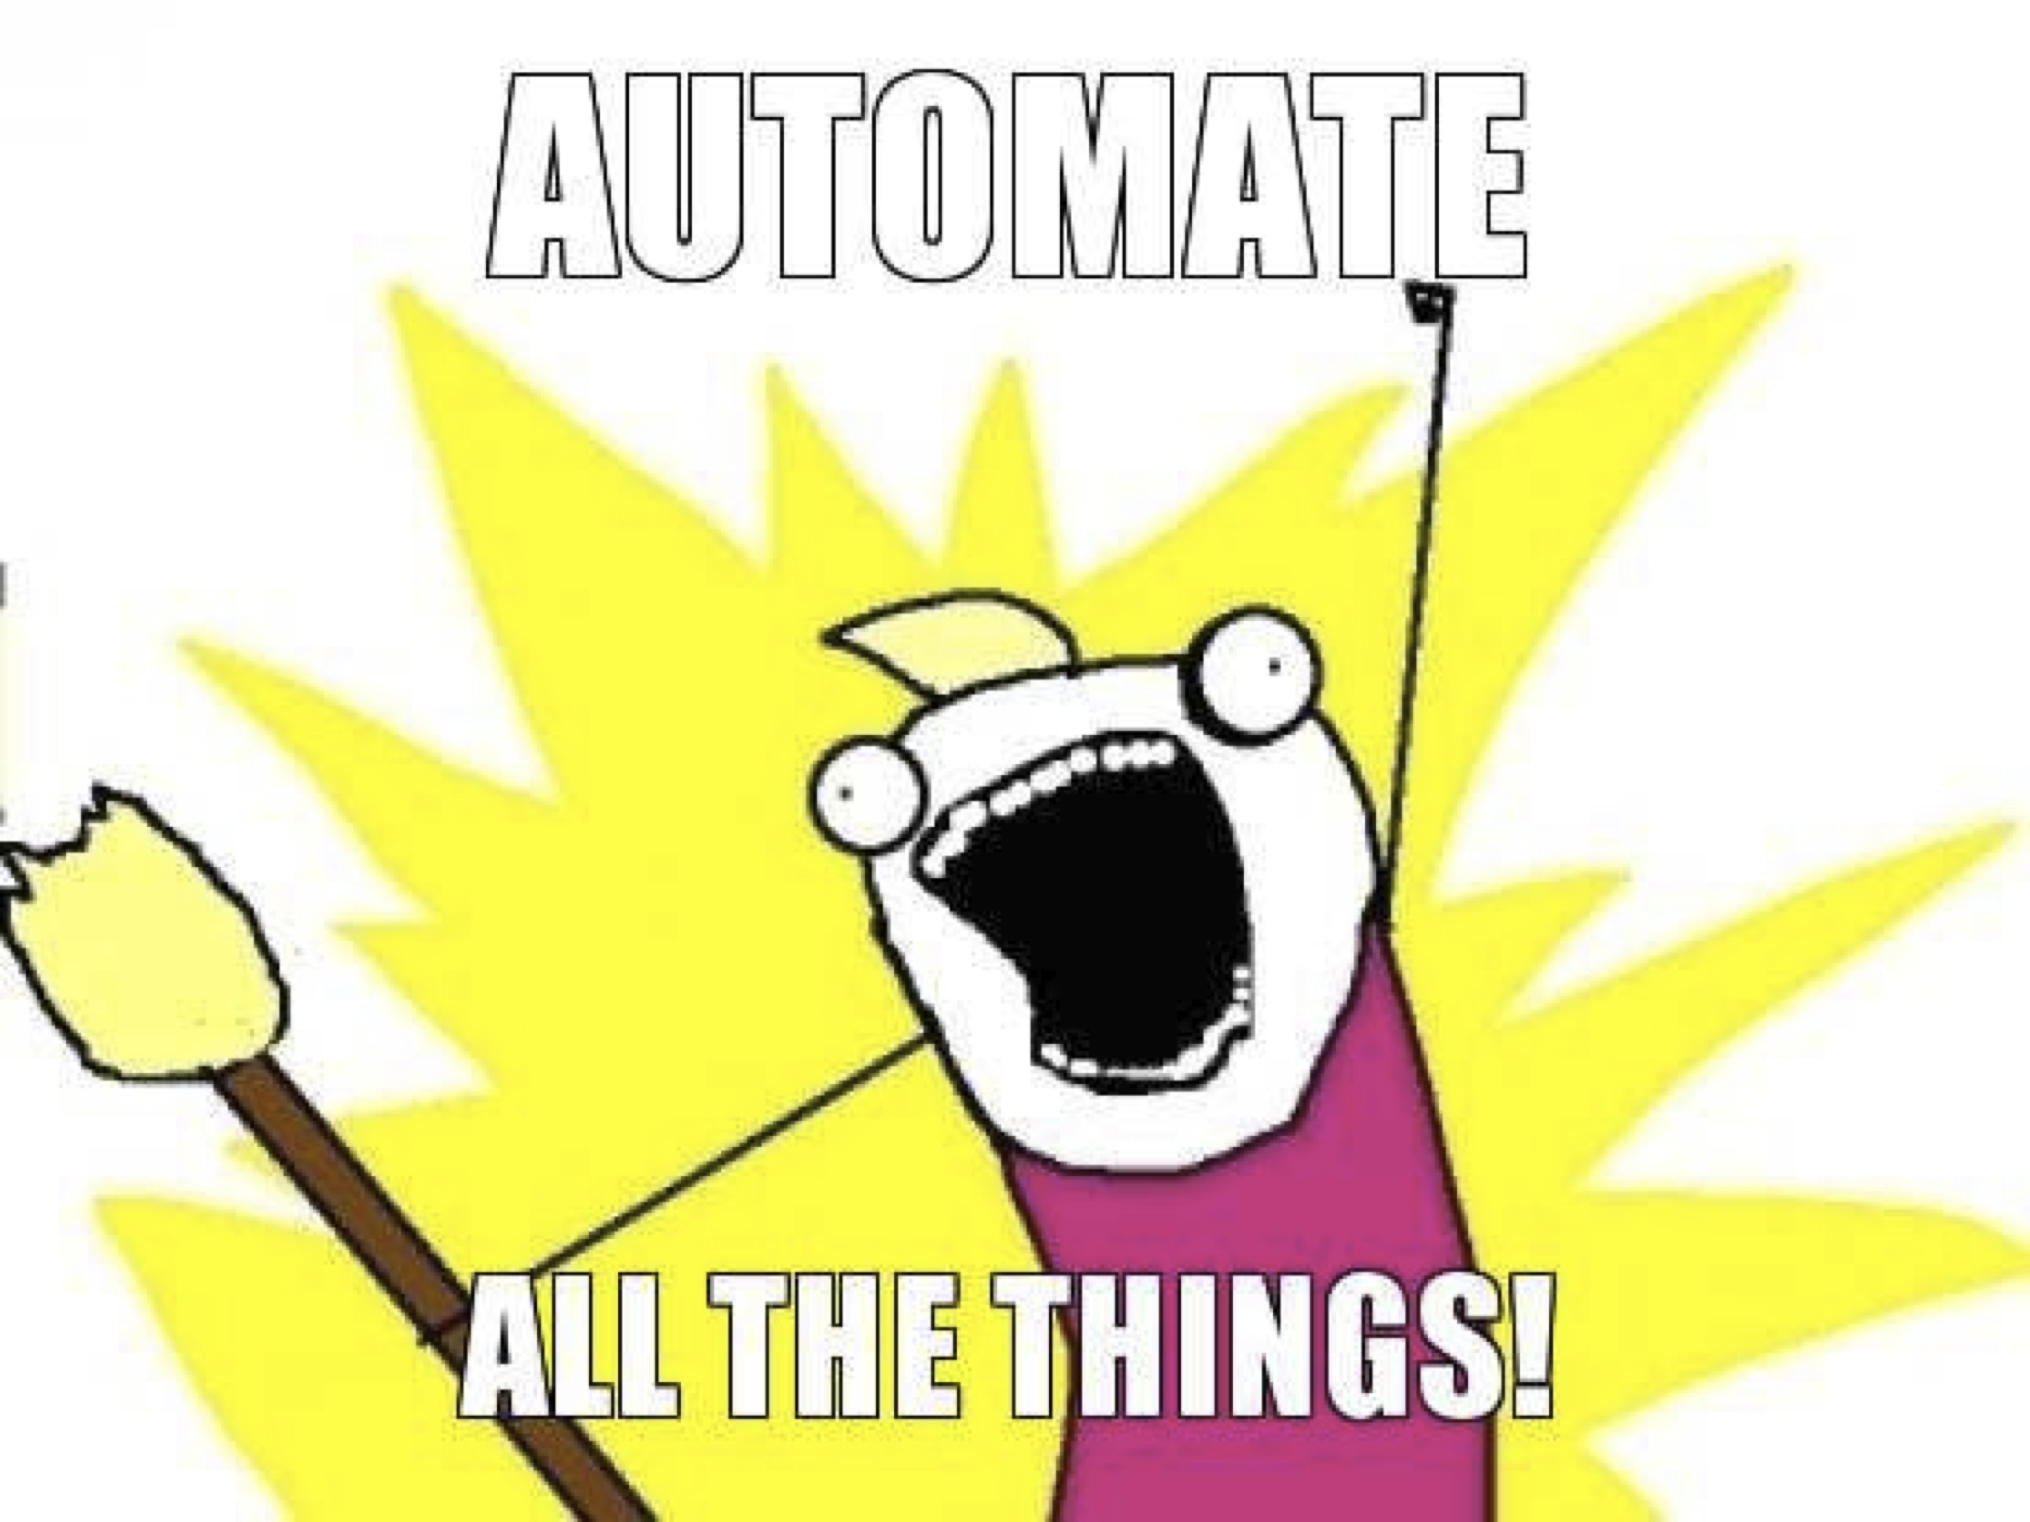
\includegraphics[width=1\textwidth]{automate-all-the-things}}
  \caption{Automate All The Things!}
  \label{fig:automate-all-the-things}
\end{figure}


\section{What doesn't Chef do?}

\begin{itemize}
  \item <<Magically>> configure your server
  \item Blindly reuse cookbooks and recipes
  \item Monitor your servers or software
  \item Undoing concept
\end{itemize}


\section{Summary}

The key underlying principle of Chef is that you (the user) knows best about what your environment is, what it should do, and how it should be maintained. The chef-client is designed to not make assumptions about any of those things. Only the individuals on the ground — that's you and your team—understand the technical problems and what is required to solve them. Only your team can understand the human problems (skill levels, audit trails, and other internal issues) that are unique to your organization and whether any single technical solution is viable.

The idea that you know best about what should happen in your organization goes hand-in-hand with the notion that you still need help keeping it all running. It is rare that a single individual knows everything about a very complex problem, let alone knows all of the steps that may be required to solve them. The same is true with tools. Chef provides help with infrastructure management, and can help solve very complicated problems. Chef also has a large community of users who have a lot of experience solving a lot of very complex problems. That community can provide knowledge and support in areas that your organization may not have and (along with Chef) can help your organization solve any complex problem.
